
%==========================================================================================================
% MULAI BAB II
%==========================================================================================================
\chapter{BASIC THEORY}
\label{chap:dasar_teori}
%==========================================================================================================
% Subbab
%==========================================================================================================
\section{\textit{Virtual Reality}} \cite{Craig}
\label{sec:VR}
When we speak of �virtual reality� (VR) we refer to a computer simulation that creates an image of a world that appears to our senses in much the same way we perceive the real world, or �physical� reality. In order to convince the brain that the synthetic world is authentic, the computer simulation monitors the movements of the participant and adjusts the sensory display or displays in a manner that gives the feeling of being immersed or being present in the simulation. Concisely, virtual reality is a means of letting participants physically engage in some simulated environment that is distinct from their physical reality. 

Virtual reality is a medium, a means by which humans can share ideas and experiences. We use the word experience to convey an entire virtual reality participation session. The part of the experience that is �the world� witnessed by the participant and with which they interact is referred to as the virtual world. However, the term �virtual world� does not only refer specifically to virtual reality worlds. It can also be used to refer to the content of other media, such as novels, movies, and other communication conventions. 

Here is a more formal definition for virtual reality from Sherman and Craig: 
A medium composed of interactive computer simulations that sense the participant�s position and actions, providing synthetic feedback to one or more senses, giving the feeling of being immersed or being present in the simulation.

Note that the definition states that a virtual reality experience provides synthetic stimuli to one or more of the user�s senses. A typical VR system will substitute at least the visual stimuli, with aural stimuli also frequently provided. A third, less common sense that is included is skin-sensation and force feedback, which is jointly referred to as the haptic (touch) sense. Less frequently used senses include vestibular (balance), olfaction (smell), and gustation (taste).

\section{\textit{Augmented Reality}}
\label{sec:AR}
Ronald Azuma in Year 1997 \cite{Azuma1997} defined Augmented Reality as a system that have characteristics:
\begin{itemize}
	\item Merger real and virtual environment
	\item Interactive in real time
	\item Registered in 3D
\end{itemize}
\textit{Augmented Reality} (AR) simply defined as real environment added with virtual object. Augmentation is done in order to enhance the users surrounding environment in real-time in respect to some function or purpose. The combination of real object and virtual object enable with appropriate display technology, interactivity enable through specific input equipments. Not like VR that fully change real environment, AR only added or complete real environment \cite{Azuma1997}. 

%AR merupakan variasi dari \textit{Virtual Environments} (VE), atau yang lebih dikenal dengan istilah \textit{Virtual Reality} (VR). Teknologi VE membuat pengguna tergabung dalam sebuah lingkungan virtual secara keseluruhan. Ketika tergabung dalam lingkungan tersebut, pengguna tidak bisa melihat lingkungan nyata disekitarnya. Sebaliknya, AR memungkinkan pengguna untuk melihat lingkungan nyata, dengan objek virtual yang ditambahkan atau tergabung dengan lingkungan nyata. Tidak seperti VR yang sepenuhnya menggantikan lingkungan nyata, AR sekedar menambahkan atau melengkapi lingkungan nyata \cite{Azuma1997}. 

%\sout{Augmented Reality (AR) is a variation of Virtual Environments (VE), or Virtual Reality as it is more commonly called. VE technologies completely immerse a user inside a synthetic environment. While immersed, the user cannot see the real world around him. In contrast, AR allows the user to see the real world, with virtual objects superimposed upon or composited with the real world. Therefore, AR supplements reality, rather than completely replacing it.}

Main purpose of AR is to create new environment with merge interactivity between real and virtual environment, so that user feel created environment is real. In other word, user feel there is no difference between AR with what they look or feel in real environment. AR can be applied for all sensory, include auditory, touch and smelling. Virtual objects show information that can not received by user with them selves sensory. This matter make AR appropriate as a tool to support perception and interaction the user with real world. Information that shown by virtual object help user do activities in real world. AR is many used in fields such as health, military, manufacture industry and also have applicated in equipments that use by many people, such as mobile phone. 

\subsection{Sejarah Singkat \textit{Augmented Reality}} \cite{SairioAR}
\label{subsec:AR_history} 
The idea of enhancing persons perception of reality dates back to the 13th century when Roger Bacon made the first recorded comment on the use of lenses, i.e. eye-glasses, for optical purposes. In 1665, an experimental scientist Robert Hooke introduced an idea of augmented senses in his book Micrographia. Ever since fiction writers, military industry and lately academic and commercial researchers have paved the road for augmented reality with an increasing effort.

The term 'virtual reality' was first introduced by Jaron Lanier, the founder of VPL Research, one of the original companies selling virtual reality systems. The term was defined as �a computer generated, interactive, three-dimensional environment in which a person is immersed� (Aukstakalnis and Blatner, 1992). Other related terms include 'Artificial Reality' by Myron Krueger in the 1970�s, 'Cyberspace' by sci-fi writer William Gibson in 1984, and, more recently, 'Virtual Worlds' and 'Virtual Environments'.}

sout{Modern augmented reality was realized for the first time in 1993. Starner (1996) wrote the first version of the Remembrance Agent which was an augmented memory software. Later that year Feiner, MacIntyre and Seligman (1993a) developed the KARMA augmented reality system. KARMA was developed to assist maintenance person with wireframe schematics and maintenance instructions on top of whatever was being repaired.}

It is not surprising that augmented reality is gaining more and more attention and research effort. This is due to the fact that until today, the requirements of feasible augmented reality applications have been out of reach of reasonably priced technology. Today, however, even the consumer technology is catching up with the requirements and opening up a plethora of new application opportunities.}

\subsection{\textit{Mixed Reality}}
\label{subsec:mixed_reality}
Augmented reality is similar to virtual reality in the sense that both make use of computer generated virtual data. Virtual reality tries to generate a complete environment, simulated or completely synthetic, that surrounds or immerses the subject. Augmented reality differs from virtual reality in that it does not try to block the surrounding real environment from user. Instead its purpose is to enhance the environment for some specific purpose \cite{SairioAR}.

Paul Milgram and Fumio Kishino formulate possible merger framework and merger real world and virtual environment which is called Milgram's Reality-Virtuality Continuum in year 1994.  From the figure \ref{fig:milgram_continuum}, at the left side is real environment that only contain real object, and at the right side is virtual environment and contain virtual object \cite{Milgram1994a}.  

\begin{figure}[h]
\begin{center}
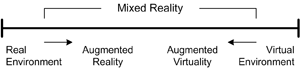
\includegraphics{./images/Milgram_Continuum}
\caption{\label{fig:milgram_continuum} Mixed Reality}
\end{center}
\end{figure}

In augmented reality, that closer to left side, environment is real and object is virtual, while in augmented virtuality, that closer to right side, environment is virtual and object is real. Augmented reality and augmented virtuality is merged and become mixed reality. The topic about AR many appear in various literature, usually that paper also study topic that have known before, that is Augmented Virtuality or well known as Virtual Reality (VR). However, today little agreement clearly about appropriate definition both for VR or AR. 

The topic of AR has begun to appear in the literature with increasing frequency, usually in conjunction with some treatment of the better known subject of Virtual Reality (VR). However, there is currently little consensus on precise definitions of either VR or AR. VR, for example, is used to refer to systems ranging from totally immersive computer generated virtual environments, to interactive desktop computer graphic applications, to text-only "Adventure" style computer games. The term "Augmented Reality" is also used in different ways by different people, without what could reasonably be considered a consistent definition. We use AR to refer to real scenes that are enhanced or "augmented" with computer graphics. Although in terms of their fundamental properties VR and AR may appear to be quite different, they face many of the same issues, and much of the research and technology of one pertains to the other \cite{Milgram1995}.

In general, a Virtual Reality environment is one in which the user is immersed in a completely synthetic world, which mimics the properties of a real-world environment to a certain extent, and which may also exceed the bounds of physical reality by creating a world in which the physical laws governing gravity, time and material properties no longer hold. In contrast, the real-world environments of Augmented Reality systems are obviously constrained by the laws of physics, which necessarily impose certain restrictions on one's ability to interact with the world. AR tools are designed to facilitate such interactions. Rather than regard the concepts of VR and AR as antitheses, however, it is more instructive to view them as lying at opposite ends of a continuum, which we refer to as the Reality-Virtuality (RV) continuum \cite{Milgram1994b}.

\section{Display Technique of Augmented Reality}
\label{sec:AR_display}
Display  system of AR is an image manipulation system that use a set of optic, electronics and mechanical components to create an image in the optic path between eye's observer and physical object merge with AR technique. Depend on optic used, image can be create on a flat object or on a complex surface (not horizontal)\cite{Bimber2005}. Figure \ref{fig:diagram_AR} ilustrate the image probability that will make to support AR, lay of display depend from the view of user and object, and the type of image is like what will earn (planar atau curved).

\begin{figure}[h]
	\centering
		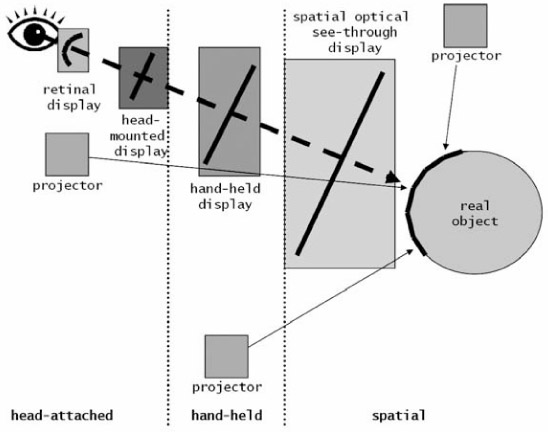
\includegraphics[width=10cm]{images/diagram_display_AR}
	\caption{Pembentukan citra untuk display \textit{augmented reality}}
	\label{fig:AR_display_diagram}
\end{figure}

There are three display AR techniques \cite{Bimber2005}, such as:

\begin{enumerate}
\item \textit{Head-Attached Display}
\item \textit{Handheld Display}
\item \textit{Spatial Display}
\end{enumerate}

\subsection {Head-Attached Display}
\label{subsec:HAD}
Head-Attached Display is a display technique that require users to use this system in the head of users. Based on the image technique formed, Head Attached Display consists of three: Virtual Retina Display which use laser with low energy to show direct image to the retina, Head-Mounted Display which use small display in front of eye, and Head-Mounted Projectors which use projector or small LCD panel and have own lights to show direct image to real environment \cite{Bimber2005}. The advance of this technique is more comfort to users, because of the image form follows user's viewpoint.

\subsubsection {\textit{Head-Mounted Display}}
\label{subsubsec:HMD}
HMD menggabungkan citra dari objek virtual dan objek nyata dan menampilkannya langsung ke mata pengguna melalui suatu alat yang dipasang di kepala pengguna. Terdapat dua tipe utama perangkat \textit{Head-Mounted Display} (HMD) yang digunakan dalam aplikasi realitas tertambah, yaitu \textit{optical-see-through} HMD dan \textit{video see-through} HMD. Keduanya digunakan untuk berbagai jenis pekerjaan dan memiliki keuntungan dan kerugian masing-masing. Dengan \textit{optical-see-through} HMD, lingkungan nyata dilihat melalui cermin semi transparan yang diletakkan di depan mata pengguna. Cermin tersebut juga digunakan untuk merefleksikan citra yang dibentuk oleh komputer ke mata pengguna, menggabungkan lingkungan nyata dan virtual. Dengan \textit{video see-through} HMD, lingkungan nyata direkam mengunakan dua kamera video yang terintegrasi ke alat, seperti gambar \ref{fig:actual_see-trough_HMD}, dan citra yang dibentuk komputer digabung dengan video tadi untuk merepresentasikan lingkungan yang akan dilihat pengguna \cite{Rolland1994}.

\begin{itemize}

\item {\textit{Video-see-through Head-Mounted Display}}

\textit{Video see-through} HMD bekerja dengan menggabungkan sebuah \textit{closed-view} HMD dengan satu atau dua \textsl{head-mounted} kamera video, melalui kamera video tersebut pengguna melihat ke lingkungan nyata. Video dari kamera dikombinasikan dengan citra yang dibuat oleh \textit{scene generator}, dunia nyata dan virtual digabungkan. Hasilnya dikirimkan ke monitor yang terletak di depan mata pengguna. Gambar \ref{fig:opaque_HMD} menunjukkan konsep dari \textit{Video see-through} HMD, gambar \ref{fig:actual_opaque_HMD} adalah contoh \textit{Video see-through} HMD, dengan dua video terintegrasi di bagian atas Helm \cite{Azuma1997}.

\begin{figure}[h!]
\begin{center}
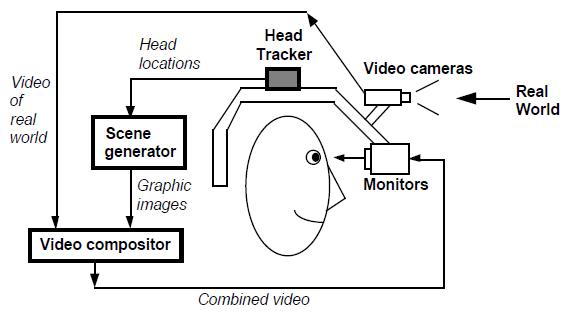
\includegraphics[width=11cm]{./images/opaque_HMD}
\caption{\label{fig:opaque_HMD} Diagram \textit{Opaque} HMD}
\end{center}
\end{figure}
\begin{figure}[h!]
\begin{center}
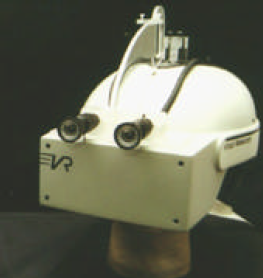
\includegraphics[width=5cm]{./images/actual_opaque_HMD}
\caption {\label{fig:actual_opaque_HMD} Contoh \textit{Opaque} HMD}
\end{center}
\end{figure}

%Ketika digunakan dengan satu mata, pengguna harus mengintegrasikan padangan dunia nyata yang diamati melalui mata yang tidak tertutup dengan pencitraan grafis yang diproyeksikan kepada mata yang satunya. Namun, ketika digunakan dengan kedua mata, pengguna mempersepsikan dunia nyata melalui rekaman yang ditangkap oleh kamera. Sebuah komputer  kemudian menggabungkan rekaman atas dunia nyata tersebut dengan pencitraan grafis untuk menciptakan efek AR yang didasarkan pada rekaman.

\item {\textit{Optical see-through Head-Mounted Display}}

Tidak seperti penggunaan \textit{video see-through} HMD, \textit{optical see-through} HMD  menyerap cahaya dari lingkungan luar, sehingga memungkinkan pengguna untuk secara langsung mengamati dunia nyata dengan mata. Selain itu, sebuah sistem cermin yang diletakaan di depan mata pengguna memantulkan cahaya dari pencitraan grafis yang dihasilkan komputer. Pencitraan yang dihasilkan merupakan gabungan optis dari pandangan atas dunia nyata dengan pencitraan grafis \cite{Azuma1997}.

\begin{figure}[h!]
\begin{center}
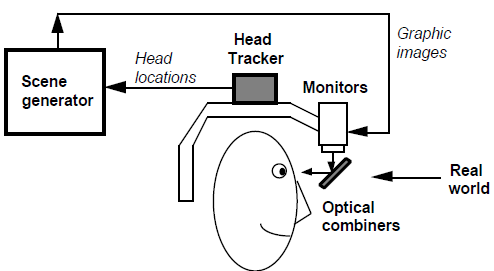
\includegraphics[width=11cm]{./images/see-trough_HMD}
\caption{\label{fig:see-trough_HMD} Diagram \textit{see-trough} HMD}
\end{center}
\end{figure}
\begin{figure}[h!]
\begin{center}
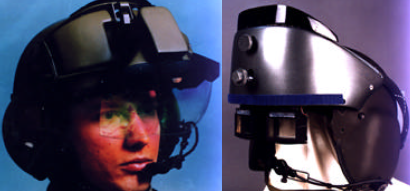
\includegraphics[width=10cm]{./images/actual_see-trough_HMD}
\caption {\label{fig:actual_see-trough_HMD} Contoh \textit{see-through} HMD, dibuat oleh Hughes Electronics}
\end{center}
\end{figure}

\end{itemize}

\subsubsection {\textit{Head-Mounted Projectors}}
\label{subsubsec:HMDP}

\subsubsection {\textit{Virtual Retina Display}}
\label{subsubsec:VRD}
Virtual retina display (VRD), atau disebut juga dengan \textit{retinal scanning display} (RSD), memproyeksikan cahaya langsung kepada retina mata pengguna\cite{Haller2010}. VRD dapat menampilkan proyeksi citra yang penuh dan juga tembus pandang tergantung pada intensitas cahaya yang dikeluarkan, sehingga pengguna dapat menggabungkan realitas nyata dengan citra yang diproyeksikan  melalui sistem penglihatannya. VRD dapat menampilkan jarak pandang yang lebih luas daripada HMD dengan citra beresolusi tinggi\cite{Jacko2010}.  Keuntungan lain VRD adalah konstruksinya yang kecil dan ringan. Namun, VRD yang ada kini masih merupakan prototipe  yang masih terdapat dalam tahap perkembangan, sehingga masih belum dapat menggantikan HMD yang masih dominan digunakan dalam bidang AR.

\begin{figure}[h]
	\centering
		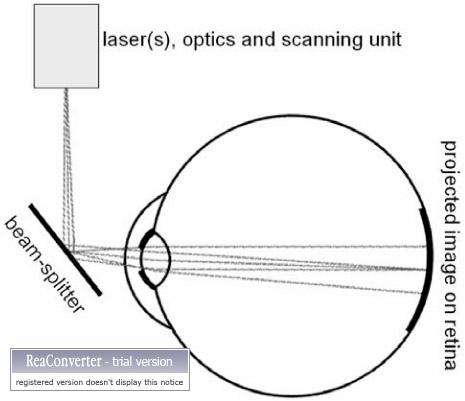
\includegraphics[width=10cm]{images/virtual_retina_diagram}
	\caption{\label{fig:VRD_diagram} Diagram sederhana \textit{virtual retina display}}
\end{figure}

%\begin{figure}[h]
%\begin{center}
%\includegraphics{./images/Vrd_blocks.gif}
%\caption{\label{fig:vrd_block} Diagram Blok \textit{Virtual Retina Display}}
%\end{center}
%\end{figure}

\subsubsection {\textit{Handheld Display}}
\label{subsubsec:handheld_display}
Teknik ini menggunakan alat dengan display yang dengan mudah dapat digenggam pengguna (Tablet PC, PDA dan telepon genggam). Sensor dapat berupa GPS, kompas digital ataupun kamera yang ada pada \textit{handheld} tersebut. Semua penerapan AR pada perangkat genggam menggunakan kamera untuk menggabungkan citra digital dengan lingkungan nyata, \textit{Handheld} AR sangat menjanjikan untuk tujuan komersial. Dua kelebihan utama dari \textit{Handheld} AR adalah mobilitas perangkat yang mudah dan salah satu perangkat genggam yang banyak digunakan (telepon genggam) telah banyak dilengkapi kamera.

\begin{figure}[h]
	\centering
		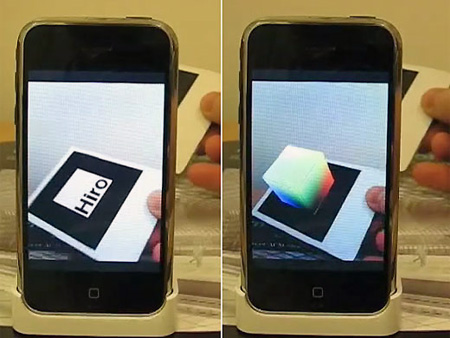
\includegraphics[width=10cm]{images/handphone_AR}
	\caption{\label{fig:AR_phone} Contoh augmented reality dengan \textit{handphone}}
\end{figure}

\subsubsection {\textit{Spatial Display}}
\label{subsubsec:spatial_display}
Dalam \textit{Spatial Augmented Reality} (SAR), objek nyata digabungkan langsung dengan citra yang terintegrasi langsung ke lingkungan nyata. Contohnya, citra diproyeksikan ke lingkungan nyata menggunakan proyektor digital atau tergabung dengan lingkungan menggunakan panel display \cite{Ramesh1998}. Perbedaan utama pada SAR dibanding teknik display sebelumnya adalah displaynya terpisah dengan pengguna. SAR memiliki kelebihan dari HMD dan handheld, sistem ini bisa digunakan oleh banyak orang pada waktu bersamaan tanpa perlu mengenakan suatu alat.

Ada tiga teknik display dalam SAR \cite{Bimber2005}, yaitu sebagai berikut:
\begin{enumerate}
\item \textit{Screen-Based Video See-Through Displays}

\textit{Screen-based }AR menggabungkan citra dan lingkungan nyata yang ditampilkan ke sebuah monitor.

\begin{figure}[h]
	\centering
		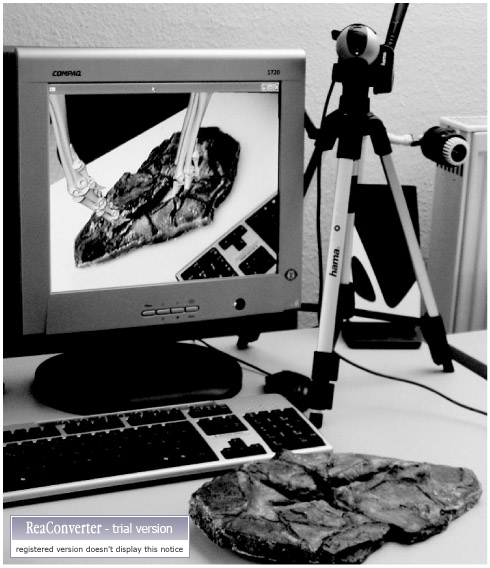
\includegraphics[width=10cm]{images/screen_SAR}
	\caption{\label{fig:SAR_screen} Contoh \textit{Screen-Based Video See-Through Displays} }
\end{figure}

\item \textit{Spatial Optical See-Through Displays}
spatial optical see-through displays generate images that are aligned within the physical environment. Spatial optical combiners, such as planar or curved mirror beam combiners, transparent screens, or optical holograms are essential components of such displays. 

\item \textit{Projection-Based Spatial Displays}
Projector-based spatial displays use front-projection to seamlessly project images directly on a physical objects' surfaces instead of displaying them on an image plane (or surface) somewhere within the viewer's visual field. Single static or steerable, and multiple projectors are used to increase the potential display area and enhance the image quality.

\end{enumerate}

\section{\textit{Tracking} Objek 3D Virtual dengan \textit{Augmented Reality}}
%\section{\textit{Augmented Reality} and 3D Object}
\label{sec:AR_with_marker}
%The AR interface combines aspects of virtual reality and the realworld environment by providing a person a chance at viewing one or more virtual 3D objects in realworld space. 
One of the disadvantages of a completely immersive virtual environment is the loss of �sense of self� in space. That is, in immersive virtual reality one�s self is composed of small components of the physical self through the use of avatars or portions of one�s body, acting in a space consisting of virtual objects. This has often resulted in feelings of disorientation and difficulty in movement and intended behaviors in the virtual environment. Active vision theory describes the importance of maintaining a sense of physical presence in order to make behaviors that are based upon information obtained moment-to-moment. 

In virtual environments experienced through a computer desktop-based application, manipulation of an object is performed through operations that ``filter'' the manipulation of an object. In other words, in order to rotate or move a virtual object, the person must cognitively ``transform'' these operations into 1) move mouse cursor over appropriate button, 2) click button, 3) see object orientation change, and 4) process the result in order to create additional mouse clicks. This brief list is greatly simplified to explain the complicated cognitive and motor processes needed in order to make a desktop virtual object change its orientation. The point is that such processes may inhibit the acquisition of visual information. Active vision theory advocates the direct physical manipulation of an object for the effective computation of object recognition and eventual understanding in accordance with this recognition. This ``filtering'' effect of desktop interfaces has been postulated to inhibit the effective cognitive processes involved in assimilating and accommodating information. Early studies of this interface have indeed shown that some ``visual affordances'' are more effectively produced with an augmented reality system than with virtual reality [26].

In AR, the person is able to combine a virtual 3D object into the normal viewing perspective without losing any of the advantages of object movement and individual movement that creates the behaviors that help us perform activity (gain sensorial-based knowledge) in real-world environments. AR enhances real scenes viewed by the user, overlaying virtual objects over the real world, and works to improve the user's performance in and perception of the world. AR has the following advantages: 1) one can get three-dimensional (3D) information based on a real scene, 2) one can see objects from their own viewpoint, and 3) one can interact with both virtual and real objects. 

Teknologi AR dapat menggabungkan interaktifitas dunia nyata dengan environment yang dibentuk komputer yang seolah-olah mereka tergabung dalam satu environment. Dengan kata lain, AR seolah-olah menggabungkan objek virtual dengan objek nyata, misalnya sebuah gambar nyata dengan pola tertentu dengan model 3D tertentu, kamera yang terhubung ke komputer  menangkap sebuah citra dari tracker yaitu gambar dengan pola tertentu. Dengan adanya pengenalan pola, sistem akan mengenali gambar tersebut. Jika pola tersebut terindentifikasi maka sistem akan menampilkan model 3D yang telah ditentukan jika pola tersebut ditemukan. Proses tersebut berlangsung secara \textit{real-time} sehingga objek virtual yang tampil di komputer akan mengikuti pergerakan \textit{tracker}.

\begin{figure}[h]
\begin{center}
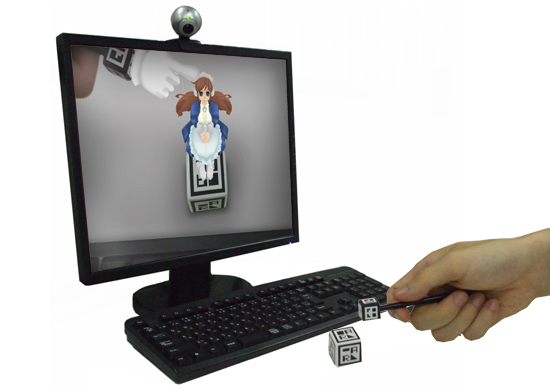
\includegraphics[width=7cm]{./images/contoh_AR}
\caption{\label{fig:contoh_AR} Aplikasi Augmented Reality Pada Game}
\end{center}
\end{figure}